\documentclass[tikz,border=10pt]{standalone}
\usepackage{tikz}
\usetikzlibrary{angles,quotes,calc}

\begin{document}
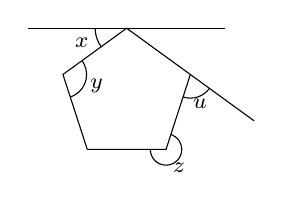
\begin{tikzpicture}[scale = 1]
    % Initial point
    \coordinate (A) at (0,0);
    % Draw octagon
    % Draw pentagon
    \draw (A) -- ++(0:1cm) coordinate (B) -- ++(72:1cm) coordinate (C) -- ++(144:1cm) coordinate (D) -- ++(216:1cm) coordinate (E) -- cycle;

    % Horizontal line
    \draw (-0.75, 52 |- D) coordinate (L) -- (1.75,52 |- D);
    % extended line
    \draw (C) -- ++(-36:1cm) coordinate (F);
    
    % Draw the angle between lines
    \pic [draw, "\footnotesize $z$ ", angle eccentricity=1.4, angle radius=0.2cm] {angle = A--B--C};
    \pic [draw, "\footnotesize $u$", angle eccentricity=1.3, angle radius=0.3cm] {angle = B--C--F};
    \pic [draw, "\footnotesize $x$", angle eccentricity=1.5, angle radius=0.4cm] {angle = L--D--E};
    \pic [draw, "\footnotesize $y$", angle eccentricity=1.5, angle radius=0.3cm] {angle = A--E--D};
    
\end{tikzpicture}
\end{document}

